\documentclass{easychair}

% \usepackage{doc}
\usepackage{setspace}
\usepackage{verbatim}
\usepackage{amssymb}
\usepackage[straightquotes]{newtxtt}

%----Suppress extra space in texttt mode
%\AddToHook{cmd/ttfamily/after}{\frenchspacing}

%----Making things more compact
\newcommand{\smalltt}[1]{\small \texttt{#1}}
\newenvironment{packed_itemize}{
\vspace*{-0.3em}
\begin{itemize}
\setlength{\partopsep}{0pt}
\setlength{\itemsep}{1pt}
\setlength{\parskip}{0pt}
\setlength{\parsep}{0pt}
}{\end{itemize}}
\newenvironment{packed_enumerate}{
\vspace*{-0.3em}
\begin{enumerate}
\setlength{\partopsep}{0pt}
\setlength{\itemsep}{1pt}
\setlength{\parskip}{0pt}
\setlength{\parsep}{0pt}
}{\end{enumerate}}
% \renewcommand{\textfraction}{0.07}
% \renewcommand{\topfraction}{0.9}
% \renewcommand{\bottomfraction}{0.9}
% \renewcommand{\floatpagefraction}{0.66}
% \setlength{\floatsep}{2.0pt plus 2.0pt minus 2.0pt}
% \setlength{\textfloatsep}{5.0pt plus 2.0pt minus 0.0pt}

\newcommand{\dav}[1]{{\color{red}{David: {#1}}}}

\title{Towards StarExec in the Cloud}

\author{
  David Fuenmayor\inst{1}
\and
  Jack McKeown\inst{2}
\and
  Geoff Sutcliffe\inst{2}
}

\institute{
  University of Bamberg,
  Bamberg, Germany\\
  \email{david.fuenmayor@uni-bamberg.de}
\and
  University of Miami,
  Miami, USA\\
  \email{jam771@miami.edu,geoff@cs.miami.edu}
}

\authorrunning{Fuenmayor, McKeown, Sutcliffe}
\titlerunning{Stars in the Clouds}

\begin{document}
\maketitle

%--------------------------------------------------------------------------------------------------
\begin{abstract}
StarExec has been central to much progress in logic solvers over the last 10 years.
It was recently announced that StarExec Iowa will be decommissioned, and while StarExec Miami 
will continue to operate while funding is available, it will not be able to support the large 
number of logic solver communities supported by the larger StarExec Iowa. 
In the long term StarExec will necessarily have to migrate to a commonly available compute 
service. 
This paper describes work being done to reengineer StarExec as a cloud-native application using
container technology and infrastructure-as-code practices.
The first step has been to containerize StarExec and ATP systems so that they can be run on a 
broad range of computer platforms. 
The next step in process is to write a new backend in StarExec so that Kubernetes can be used to 
orchestrate distribute of StarExec job pairs over whatever compute nodes are available.
One possibility is to host StarExec-Kubernetes in AWS.
\end{abstract}
%--------------------------------------------------------------------------------------------------
% Geoff
\section{Introduction}
\label{Introduction}

Automated Theorem Proving (ATP) is concerned with the development and use of tools that automate 
sound reasoning: the derivation of conclusions that follow inevitably from facts.
Automated Theorem Proving (ATP) is at the heart of many computational tasks, in particular for
verification \cite{Har06,HH19} and security \cite{Coo18}.\footnote{%
In AWS -
\href{https://aws.amazon.com/what-is/automated-reasoning/}{\tt aws.amazon.com/what-is/automated-reasoning/}, 
\href{https://aws.amazon.com/security/provable-security//}{\tt aws.amazon.com/security/provable-security/}.} 
New and emerging application areas include
chemistry \cite{Yad17}, 
biology \cite{CC+13}, 
medicine \cite{HLB05},
elections \cite{Nip09,BDS17}, 
auctions \cite{CK+15}, 
privacy \cite{Lib20},
law \cite{PS15}, 
ethics \cite{DF+16}, 
religion \cite{OZ11,BW14-ECAI,Hor19},
and business \cite{Han98}.
ATP systems are also used as components of more complex Artificial Intelligence (AI) systems,
and the impact of ATP is thus extended into many facets of society.
% in areas such as 
% knowledge representation \cite{TR+04}, 
% natural language processing \cite{BM05}, 
% planning \cite{NV07}, 
% agents \cite{TBP03}, 
% commonsense reasoning \cite{MS05}, 
% and the semantic web \cite{McG04}.

The Thousands of Problems for Theorem Provers (TPTP) World \cite{Sut24} is a well established 
infrastructure that supports research, development, and deployment of ATP systems.
The TPTP World includes 
the TPTP problem library \cite{Sut17},
the TSTP solution library \cite{Sut10},
standards for writing ATP problems and reporting ATP solutions \cite{SS+06,Sut08-KEAPPA},
tools and services for processing ATP problems and solutions \cite{Sut10},
and it supports the the annual CADE ATP System Competition (CASC)~\cite{Sut16}.
Since its first release in 1993 the ATP community has used the TPTP World as an appropriate and 
convenient infrastructure for ATP system development, evaluation, and application.
The TPTP World has a diverse, engaged, and sustained user community, with various parts of the 
TPTP World being deployed in a range of applications in both academia and industry.\footnote{%
TPTP has contributed to recognized research in 627 publications that cite \cite{Sut17},
according to Google Scholar.}
The web page \href{https://www.tptp.org}{\tt www.tptp.org} provides access to all components.

The TPTP problem library was motivated by the need to provide support for meaningful ATP system 
evaluation.
This need was also (or became) evident in other logic solver communities, e.g., 
SAT~\cite{HS00-SATLIB} and SMT~\cite{BST10}.
For many years testing of logic solvers was done on individual developer's computers. 
In 2010 a proposal for centralised hardware and software support was developed,
and in 2011 a \$2.11 million NSF grant\footnote{%
NSF Awards 1058748 and 1058925, led by Aaron Stump and Cesare Tinelli at the University of Iowa} 
was obtained.
This grant led to the development and availability of StarExec Iowa~\cite{SST14} in 2012,
and a subsequent \$1.00 million grant\footnote{%
NSF Award 1730419} in 2017 expanded StarExec to Miami.
StarExec has been central to much progress in logic solvers over the last 10 years, supporting
16 logic solver communities, used for running many annual competitions~\cite{BB+19}, and 
supporting many many users.
StarExec Iowa provides community infrastructure for many logic solver communities,
e.g., ASP, QBF, SAT, SMT, Termination, etc, while
StarExec Miami is used by the TPTP community.
StarExec Miami has features that take advantage of TPTP standards, and is also used to host CASC.

It was recently announced that StarExec Iowa will be decommissioned. 
The maintainer of StarExec Iowa explained that ``the plan is to operate StarExec as usual for 
competitions Summer 2024 and Summer 2025, and then put the system into a read-only mode for one 
year (Summer 2025 to Summer 2026)''.
The 2017 grant for StarExec Miami paid for the hardware and three years of system administration.
The hardware is still hosted by the University of Miami High Performance Computing group,
funded on a shoe-string budget by the TPTP World.
While StarExec Miami will continue to operate while funding is available, it will not be able
to support the large number of logic solver communities supported by the larger StarExec Iowa.
In the long term StarExec will necessarily have to migrate to a commonly available compute service.
This paper describes work being done to reengineer StarExec as a cloud-native application using
container technology and infrastructure-as-code practices.
The first step has been to containerize\footnote{%
Strictly, ``images'' are built, and the images are deployed in containers. 
But keeping with common use of the terminology, we just say ``container'' and ``containerize''.} 
StarExec and ATP systems so that they can be run on a broad range of computer platforms.
The next step in process is to write a new backend in StarExec so that Kubernetes can be used to
orchestrate distribute of StarExec job pairs over whatever compute nodes are available.
Additionally, this work aims to build a Kubernetes backend in StarExec so that Kubernetes can
be used to orchestrate distribute of StarExec job pairs over whatever compute nodes are available.
One possibility is to host StarExec-Kubernetes in AWS.
\dav{We could say something like: supported by an AWS AR grant, we will implement the proposed approach by deploying a new (re-engineered) version of StarExec in AWS. This StarExec instance will not only be fully functional to the community (e.g. run  SystemOnTPTP, CASC competitions, etc. as much as our budget allows), but shall also serve as a an exemplary implementation (IaC template) for those willing to deploy their own (possibly customized) StarExec in their own infrastructure (cloud or on-premises).}

\dav{We shall also note that podman and kubernetes can/will both serve as backends for StarExec (the podman team keeps adding basic orchestration functionalities, so it can work as a lightweight alternative to k8s in simple scenarios). Btw podman is designed to play well with k8s (e.g. it understands k8s yaml config) so there is no big overhead in supporting both I think (this might facilitate adoption, specially since k8s still keeps some of its reputation as being very complex).}

\paragraph{This paper is organized as follows:}
Section~\ref{Background} provides a short background to ATP systems, StarExec, and 
containerization.
Section~\ref{ContainerizingStarExec} describes how StarExec has been containerized, and
Section~\ref{ContainerizingATPSystems} describes how ATP systems have been containerized.
Section~\ref{StarExecK} explains how we plan to deploy the containerized StarExec
and ATP systems in a Kubernetes setting.
Section~\ref{Conclusion} concludes and look forward to future work.

%--------------------------------------------------------------------------------------------------
\section{Background}
\label{Background}

%--------------------------------------------------------------------------------------------------
\subsection{ATP Systems}
\label{ATPSystems}

ATP Systems are complex pieces of software, typically using advanced data structures~\cite{Sch13}, 
sophisticated algorithms~\cite{Vor01}, and tricky code optimizations\cite{Sch06}.
They are written in a variety of programming languages: Prolog~\cite{Ott23,Hol23}, 
Scala~\cite{SB18}, C~\cite{SCV19}, C++~\cite{RV02-AICOMM}, OCaml~\cite{Kor06}, Python~\cite{SP20}, 
etc.
Their build processes include techniques such as parser generators~\cite{Ste21}, Makefiles,
code repositories, specific versions of libraries, etc.
For a user who is focussed on an application of ATP
% , e.g. (with a few exemplar references), in 
% mathematics \cite{Qua92-Book,MP96}, logic~\cite{GO86,Jec95}, management~\cite{PB+92-TR,PM94}, 
% planning \cite{SE94}, 
installing an ATP system can be a deal breaker, and many early users selected a weaker system, 
e.g., Otter~\cite{McC03-Otter}, for their experiments because it was readily available and easy 
enough to install.
% As the TPTP World evolved it was clear that more powerful ATP systems were available, especially
% evident in the CADE ATP System Competition (CASC)~\cite{Sut16}.
% However, these more powerful systems were often not as easy to obtain and install.
% This was a key motivation for the creation of the SystemOnTPTP service~\cite{Sut00-CADE-17}.
% SystemOnTPTP allows users to
% The ATP systems in SystemOnTPTP are installed by the third author, often with help from the
% individual system developers.
There have been some proposals for standardising the ATP system build process, e.g.,
\href{https://tptp.org/Proposals/SystemBuild.html}{\tt tptp.org/Proposals/SystemBuild.html}, 
but the diversity of ATP system software makes conformity nigh impossible.
An alternative is to push the task back on the system developers, and one approach to this is
containerizing the ATP systems, as discussed in Section~\ref{Containerization}.

%--------------------------------------------------------------------------------------------------
\subsection{StarExec}
\label{StarExec}

The need to provide support for meaningful system evaluation has been recognized in many logic 
solver communities, e.g., TPTP~\cite{SS01}, SAT~\cite{HS00-SATLIB}, SMT~\cite{CSW15},
Termination~\cite{MZ07}, etc.
For many years testing of logic solvers was done on individual developer's computers. 
In 2010 a proposal for centralised hardware and software support was developed,
and in 2011 a \$2.11 million NSF grant\footnote{%
NSF Awards 1058748 and 1058925, led by Aaron Stump and Cesare Tinelli at the University of Iowa} 
was obtained.
This grant led to the development and availability of StarExec Iowa~\cite{SST14} in 2012,
and a subsequent \$1.00 million grant\footnote{%
NSF Award 1730419} in 2017 expanded StarExec to Miami.
StarExec has been central to much progress in logic solvers over the last 10 years, supporting
16 logic solver communities, used for running many annual competitions~\cite{BB+19}, and 
supporting many many users.

Figure~\ref{ArchitectureS} shows the architecture of the currently deployed StarExec.
The hardware consists of a single head node and multiple compute nodes.
The head node provides the browser interface for users, in particular it accepts job requests
that generate job pairs consisting of an ATP system and a problem file, and distributes the
pairs to the compute nodes using the SUN Grid Engine (SGE).
\dav{Maybe we can explain which roles is SGE taking here (batch/job scheduling, cluster management, etc). I have seen also OAR as backend... }
(For development and testing, the head node can also run job pairs itself using a local backend.)
The head node maintains a relational MariaDB database, and all the nodes access an NFS mounted
shared file system.
The database records everything, including the ATP systems' files and the problem files in the 
file system.
Job pairs executing on a compute node have their time and memory usage limited and reported
by the {\tt runsolver}~\cite{\cite{Rou11}} utility (the {\tt BenchExec}~\cite{BLW19} utility in 
StarExec Iowa).
The results and resource usage data from completed job pairs are stored in the file system, 
and recorded in the database.
The browser interface provides the necessary facilities to upload ATP systems, upload problem
files, browse the ATP systems and problems, create jobs, track job progress, browse and download
job results, and delete ATP systems, problems, jobs, etc.

\begin{figure}[htb]
\begin{center}
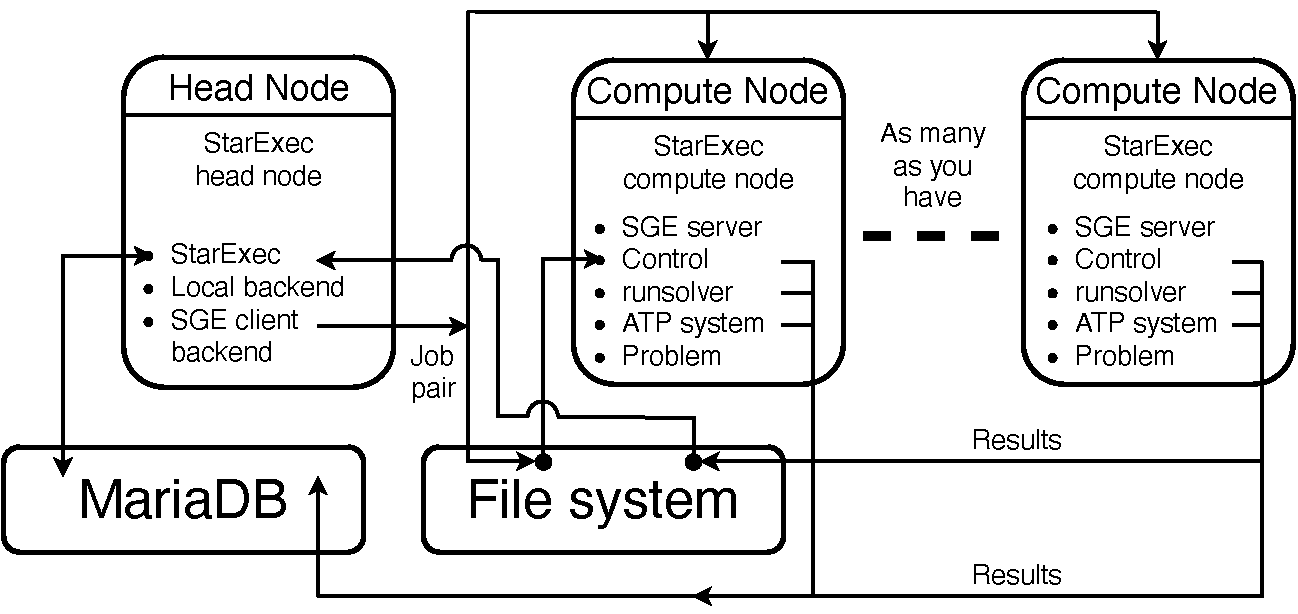
\includegraphics[width=0.8\textwidth]{ArchitectureS}
\caption{StarExec Architecture}
\label{ArchitectureS}
\end{center}
\end{figure}

It was recently announced that StarExec Iowa will be decommissioned. 
The maintainer of StarExec Iowa explained that ``the plan is to operate StarExec as usual for 
competitions Summer 2024 and Summer 2025, and then put the system into a read-only mode for one 
year (Summer 2025 to Summer 2026)''.
While StarExec Miami will continue to operate while funding is available, but it will not be able
to support the large number of logic solver communities that use the larger StarExec Iowa cluster.
In the long run it will be necessary for StarExec users to transition to new environments,
and several plans are (at the time of writing) being discussed.
One effort is that described in the paper.

%--------------------------------------------------------------------------------------------------
\subsection{Containerization}
\label{Containerization}

{\em This section was written with the help of ChatGPT~3.5.}
\dav{I will rewrite this section}

Containerization is a technology that allows developers to package an application and its 
dependencies into a standardized unit called a container. 
These containers encapsulate the application code, runtime, libraries, and other necessary 
components, providing a consistent and isolated environment for running the application 
across different computing environments.
One of the key benefits of containerization is its ability to abstract away the underlying 
infrastructure. 
Containers are designed to be lightweight and portable, making it easy to deploy applications 
across various platforms, such as laptops, servers, virtual machines, and cloud environments. 
This portability ensures that applications behave consistently regardless of the underlying 
infrastructure, simplifying the development and deployment process.
Furthermore, containerization offers several advantages in terms of scalability, resource 
efficiency, and security. 
Containers share the host operating system's kernel, which reduces overhead compared to 
traditional virtualization techniques. 
As a result, containers can be started and stopped quickly, allowing for rapid scaling of 
applications to meet changing demand. 
Containers provide a level of isolation that helps prevent conflicts between applications and 
enhances security by limiting the impact of potential vulnerabilities.

Popular containerization platforms like Docker, Podman, and Kubernetes have played a significant 
role in popularizing container technology. 
These platforms provide tools for building, distributing, orchestrating, and managing containers 
at scale. 
Docker, for example, introduced a user-friendly interface and a standardized format for defining 
container images, making it easier for developers to adopt containerization in their workflow. 
Kubernetes, on the other hand, focuses on container orchestration and automating the deployment, 
scaling, and management of containerized applications in production environments.

%--------------------------------------------------------------------------------------------------
% Jack
\section{Containerizing StarExec}
\label{ContainerizingStarExec}

%A containerized StarExec can be used locally in Docker/Podman/Kubernetes. 
%This allows StarExec users to build and test StarExec installation packages on their own computers before deploying to the StarExec Miami installation.

\dav{On justifying this effort: Containerizing StarExec components feels natural as a first step towards making it 'cloud-native'... and so on}
	
\dav{The stuff below was moved from Section \ref{StarExecK}. I think it belongs here. In this section we can comment on what we have done so far (putting current StarExec as a whole in a single container). However, a professional solution will have to split components in different (communicating) containers (two obvious candidates being the database and the batch scheduler SGE). In k8s, the StarExec components/containers would run together as a single pod. In podman we can also group containers in a similar way (analogous to docker compose).}

StarExec (see Section~\ref{StarExec}) is based around a head node that coordinates activities, 
in particular the creation of jobs as sets of job pairs, with each pair consisting of an ATP 
system and a problem. 
MariaDB is used to store job information and results, and NFS is used to share disk space between 
the head node and compute nodes. 
StarExec currently offers two backends for running job pairs: the local backend runs pairs on 
the same computer as the head node, and the Sun Grid Engine (SGE) backend sends pairs out to 
compute nodes. 

\dav{A related idea is that, following the IaC approach, the resulting sources (shell scripts, config files, Dockerfiles, etc) can be made available (e.g. as a public Git repository) to a community of users/developers, so they can build, test (and run) their own (e.g. forked) StarExec(s). This also enables people to become contributors of other StarExec repos (e.g. Miami's) by sending pull requests or the like. I think this is a good means to promote the survival of StarExec as a decentralized open-source project.}

All the files for containerizing StarExec are available from~\ldots \\
\hspace*{1cm}\href{https://github.com/StarExecMiami/starexec-containerized}{\tt github.com/StarExecMiami/starexec-containerized}\\

%--------------------------------------------------------------------------------------------------
\section{Containerizing ATP Systems}
\label{ContainerizingATPSystems}

\dav{Again, we shall justify why we are doing this. In a sense, containerizing ATPs is independent from containerizing StarExec (or making it 'cloud-native'). Of course, both efforts play well together...
It would be great for us if ATP developers become super enthusiastic about containerizing their babies after reading this section ;)}

The ATP systems' are containerized in a hierarchy, show in Figure~\ref{ImageDAG}.
The underlying operating system is {\tt ubuntu:latest} from {\tt dockerhub}~\ldots\\
\hspace*{1cm}\href{https://hub.docker.com/_/ubuntu}{\tt hub.docker.com/\_/ubuntu} \\
{\tt ubuntu-build} adds to {\tt ubuntu:latest} using {\tt apt-get} to install common software such 
as {\tt cmake}, {\tt git}, {\tt tcsh}, {\tt python3}, and {\tt wget}.
{\tt ubuntu-build} also creates an {\tt artifacts} directory where the components required for 
an ATP system execution are placed.

{\tt tptp-world-build} provides utilities from the TPTP World \cite{Sut24} that are used by 
ATP systems, e.g., {\tt SPCForProblem} detects the Specialist Problem Class (SPC) \cite{SS01} of 
a problem that is used by some ATP systems to decide on what search parameters to use.
Additionally, the {\tt runsolver} utility for limiting and reporting the resources
used by an ATP system is added.
To support these utilities some libraries that are not part of the {\tt ubuntu-build} have
to be added.
The {\tt /benchmark} directory, where the TPTP problem for the ATP system to solve is placed, is
created as part of this container.

On top of {\tt ubuntu-build} are the individual ATP system's {\em ATP-system-name}{\tt-build}
containers, and on top of that and {\tt tptp-world-build} are the final 
{\em ATP-system-name}{\tt -runsolver} containers.
The details of building the {\em ATP-system-name}{\tt -*} containers are provided below.

The {\em ATP-system-name}{\tt -runsolver} containers are pushed to {\tt dockerhub} in~\ldots\\
\hspace*{1cm}\href{https://hub.docker.com/repositories/tptpstarexec}{\tt hub.docker.com/repositories/tptpstarexec}\\
which has a directory for each ATP system.
The pushed containers are tagged as 
{\em ATP-system-name}{\tt :}{\em ATP-system-version}{\tt -runsolver-}{\em architecture},
where {\em architecture} is, e.g., {\tt arm64} or {\tt amd64}.
All the files for containerizing the ATP system are available from~\ldots \\
\hspace*{1cm}\href{https://github.com/StarExecMiami/starexec-kubernetes/tree/main/images}{\tt github.com/StarExecMiami/starexec-kubernetes/tree/main/images}\\
A {\tt Makefile} to containerize E, Leo-III, and Vampire is included.

\begin{figure}[htb]
\begin{center}
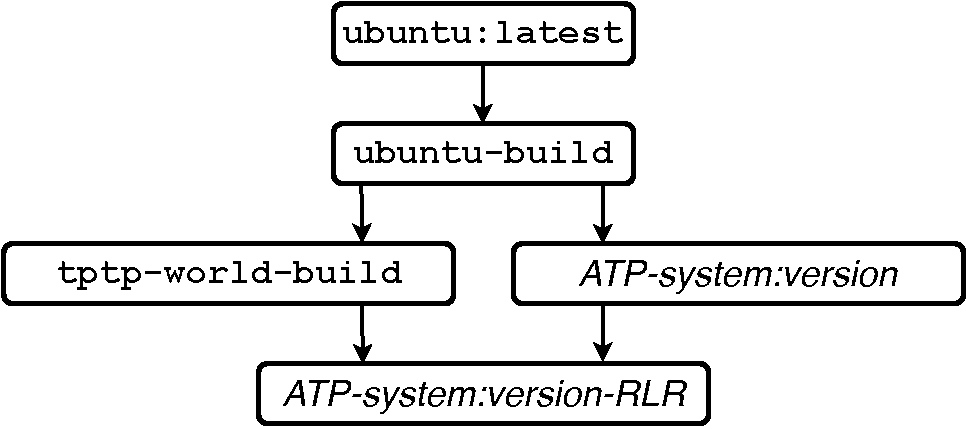
\includegraphics[width=0.8\textwidth]{ImageDAG} 
\caption{ATP System Container Hierarchy}
\label{ImageDAG}
\end{center}
\end{figure}

%--------------------------------------------------------------------------------------------------
\subsection{Containerizing ATP Systems}
\label{BuildingATPSystemImages}

Each {\em ATP-system-name}{\tt-build} adds the ATP system's executables to {\tt ubuntu-build}.
The ATP system is retrieved online, e.g., from a GitHub repository, and the necessary commands
to build the executables are run.
The executables are copied into the {\tt /artifacts} directory.
The choice of which version of the ATP system to containerize is made inside the {\tt Dockerfile},
e.g., in Figure~\ref{E---build} {\tt E 3.0.03} is chosen.
This localization is necessary because the incantations for selecting and retrieving an
particular ATP system version vary from system to system.
By convention the container is named {\em ATP-system-name}{\tt -build}, and by default has
the {\tt :latest} tag,
Figure~\ref{E---build} shows the {\tt Dockerfile} for E's {\tt -build}, using the command 
{\tt podman~build~-t~eprover-build~.}.

\begin{figure}[htb]
{\small
\begin{verbatim}
#------------------------------------------------------------
FROM ubuntu-build

# Clones repository
ARG E_VERSION=E-3.0.03
RUN git clone --depth 1 --branch $E_VERSION https://github.com/eprover/eprover.git

# Set working directory to cloned sources directory
WORKDIR /eprover

# Builds first-order executable
RUN ./configure --bindir=/artifacts && \
    make && \
    make install
# RUN cp PROVER/eprover /artifacts/eprover

# Builds higher-order executable
RUN ./configure --enable-ho && \
    make rebuild
RUN cp PROVER/eprover-ho /artifacts/eprover-ho
#------------------------------------------------------------
\end{verbatim}
}
\caption{The {\tt Dockerfile} for E's {\tt -build}}
\label{E---build}
\end{figure}

Each {\em ATP-system-name}{\tt -runsolver} is based on {\em ATP-system-name}{\tt-build} and 
{\tt tptp-world-build}.
{\em ATP-system-name}{\tt -runsolver} adds the {\tt runsolver} utility to limit and report
the resource usage of the ATP system.
Note how the containerization uses the default {\tt :latest} tagged 
{\em ATP-system-name}{\tt-build}. 
The executables from {\em ATP-system-name}{\tt -runsolver} are copied from its 
{\tt /artifacts} directory into this container's {\tt /artifacts} directory.
Additionally, the {\tt run\_system} script, described in Section~\ref{Running}, is copied into
{\tt /artifacts}.
By convention this container is named
{\em ATP-system-name}{\tt :}{\em ATP-system-version}{\tt -runsolver}, i.e., including the version
number so that users know what version of the ATP system has been containerized.
Figure~\ref{E---runsolver} shows the {\tt Dockerfile} for building E's {\tt -runsolver},
using the command {\tt podman~build~-t~eprover:3.0.03-runsolver~.}, i.e., it contains
E version {\tt 3.0.03}.

\begin{figure}[htb]
{\small
\begin{verbatim}
#------------------------------------------------------------
FROM eprover-build AS builder
FROM tptp-world-build

ENV PATH=".:${PATH}"
WORKDIR /artifacts

# E-specific stuff from ostensibly external image
COPY --from=builder /artifacts/eprover /artifacts/
COPY --from=builder /artifacts/eprover-ho /artifacts/

# run_image script 
ADD run_image /artifacts/

# run_E script 
ADD run_E /artifacts/

ENTRYPOINT ["runsolver"]
#------------------------------------------------------------
\end{verbatim}
}
\caption{The {\tt Dockerfile} for E's {\tt -runsolver}}
\label{E---runsolver}
\end{figure}

%--------------------------------------------------------------------------------------------------
\subsection{Running ATP System Containers}
\label{Running}

A Python script {\tt run\_image.py} is available to run a containerized ATP system from the 
command line.
The script is shown in Appendix~\ref{runsystem}.
Minimally the script must have the {\em ATP-system-name}{\tt -runsolver} as a command 
line argument.
By default {\tt run\_image.py} runs the {\em ATP-system-name}{\tt -runsolver} in a
{\tt podman} container, taking the problem from {\tt stdin}, imposing CPU and wall clock time 
limits of 60s, imposing no memory limit, with the intention that the ATP system should try prove 
that the problem's conjecture is a theorem.
The problem file is passed into the running container using Podman volume mounting, copying the
problem to the {\tt /artifacts/CWD/benchmark} file inside the container.
All the parameters can be changed via command line options to {\tt run\_image.py}.

The entrypoint in {\em ATP-system-name}{\tt -runsolver} is the {\tt runsolver} utility, 
which in turn starts the {\tt run\_system} script with the problem, CPU limit, wall clock limit, 
memory limit, and the proof request as arguments.
Each {\tt run\_system} script is responsible for starting theat ATP system -- this action varies 
tremendously between ATP systems, and is thus usually provided by the system developer.
For example, E has its own script {\tt run\_E} that invokes the {\tt eprover} or {\tt eprover-ho}
binary depending on whether the problem is first-order or higher-order, and depending on the
intention passed in appropriate command line arguments are given to the selected binary along
with the problem file and time limit.

%--------------------------------------------------------------------------------------------------
\section{Towards a Cloud-native StarExec}
\label{StarExecK}

\dav{Changed the title. I will work on this section soon. The idea is to sell the part on re-engineering StarExec to support two backends: podman and k8s. There will be a final section on an exemplary 'reference' deployment on AWS using their managed k8s infrastructure (EKS, etc.)}

\dav{recall StarExec current architecture}

This structure is inflexible, and must be configured to the specific hardware available. 
The plan is to use a containerized StarExec (see Section~\ref{ContainerizingStarExec}), replace 
SGE with Kubernetes, remove any MariaDB-specific bindings so that other database products can be 
used, and use containerized ATP systems (see Section~\ref{ContainerizingATPSystems}).
Figure~\ref{ArchitectureK} shows the generic architecture.

\begin{figure}[htb]
\begin{center}
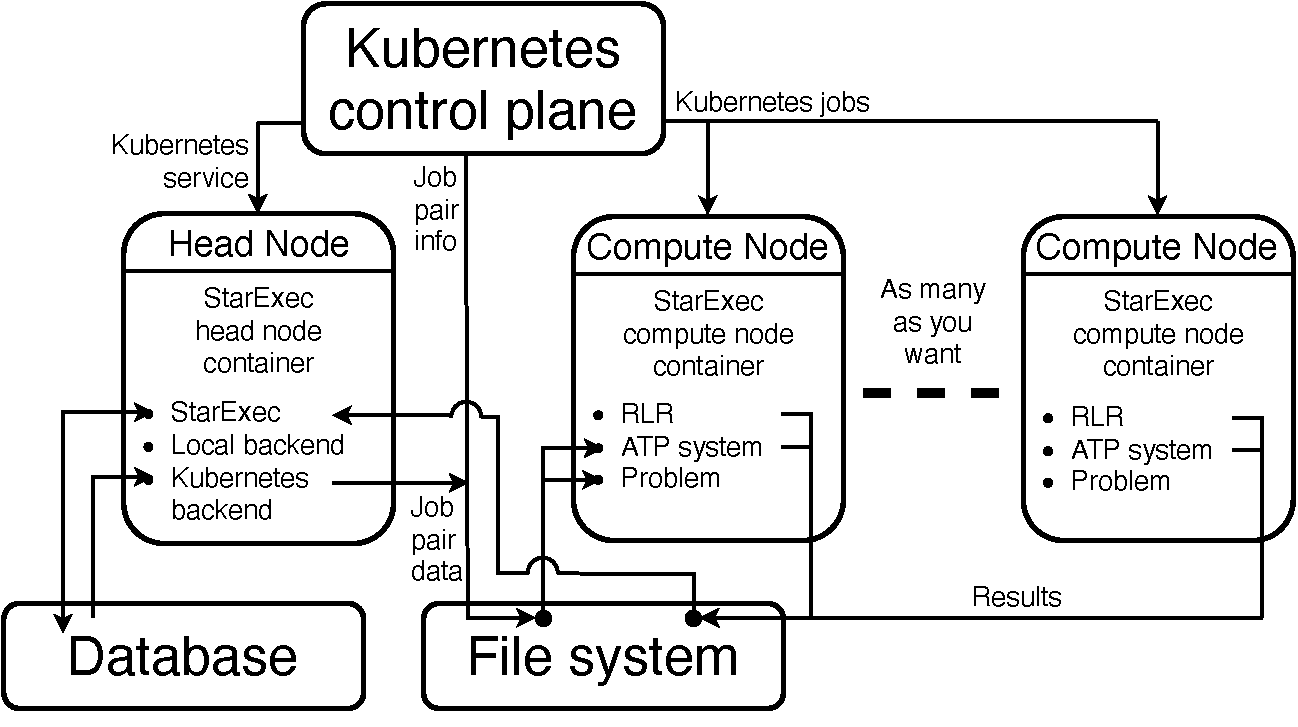
\includegraphics[width=0.8\textwidth]{ArchitectureK}
\caption{Architecture in Kubernetes}
\label{ArchitectureK}
\end{center}
\end{figure}

An Amazon Research Award\footnote{%
Amazon Research Award, Fall 2023. Any opinions, findings, and conclusions or recommendations 
expressed in this material are those of the authors, and do not reflect the views of Amazon.} 
has been granted to implement StarExec with Kubernetes in AWS.
This instantiates the the generic implementation as follows:
\begin{packed_itemize}
\item The Kubernetes host will be Amazon Elastic Kubernetes Service (EKS)
\item The head and compute nodes will be Amazon EC2 nodes.
\item The database will be Amazon Relational Database (RDS).
\item The file system will be Amazon Elastic File System (EFS).
\item The ATP systems' containerization will be made compatible with (possibly be exactly) the 
      Amazon Trusted Solver (ATS) format.
\end{packed_itemize}

The entire migration of StarExec into AWS will be done using the ``infrastructure-as-code'' 
paradigm, using Amazon CloudFormation. 
The implementation will be tested by copying the TPTP community from StarExec Miami onto the 
new StarExec AWS.
Figure~\ref{ArchitectureAWS} shows the AWS-specific architecture.

\begin{figure}[htb]
\begin{center}
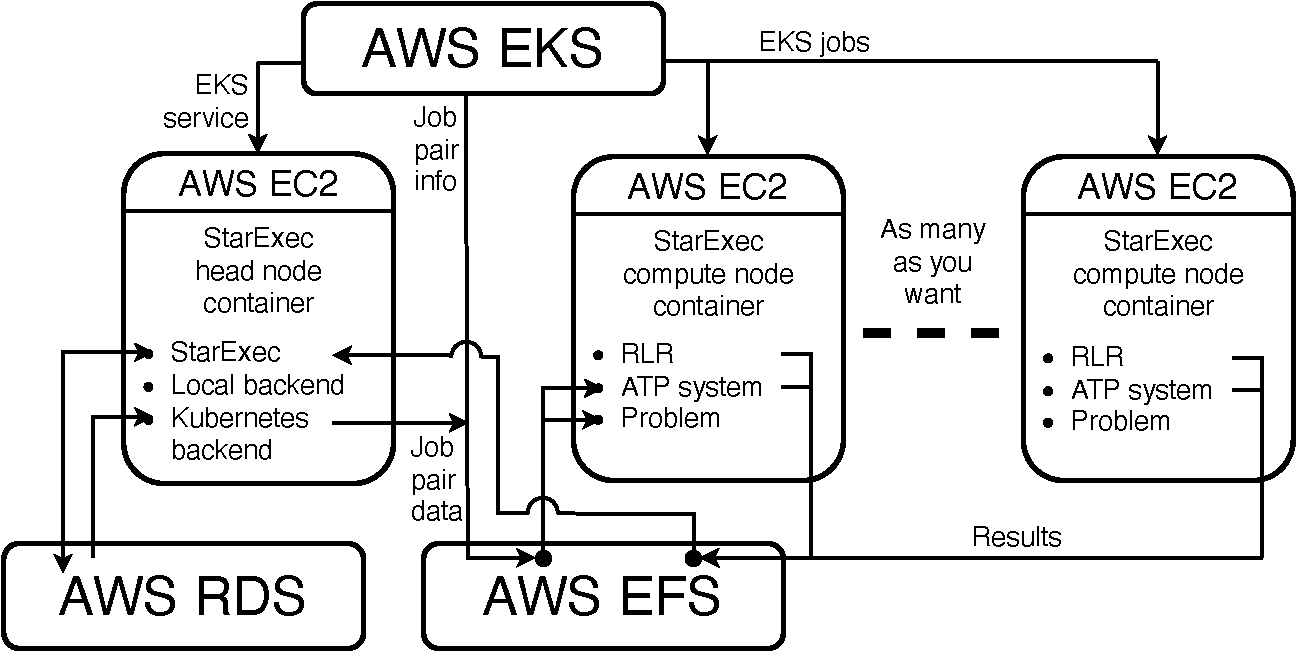
\includegraphics[width=0.8\textwidth]{ArchitectureAWS}
\caption{Architecture in EKS on AWS}
\label{ArchitectureAWS}
\end{center}
\end{figure}

%--------------------------------------------------------------------------------------------------
% Geoff
\section{Conclusion}
\label{Conclusion}

This paper has described work being done to containerize StarExec and ATP systems so that they 
can be run on a broad range of computer platforms.
Additionally, this work explains plans to build a Kubernetes backend in StarExec so that 
Kubernetes can be used to orchestrate distribute of StarExec job pairs over whatever compute 
nodes are available.

This is ongoing work -- some of the work is still ``in progress'', particularly embedding
StarExec in Kubernetes on AWS.
Hopefully the future will include StarExec being flexibly available in online compute clusters.

%--------------------------------------------------------------------------------------------------
\bibliographystyle{plain}
\bibliography{Bibliography.bib}
%--------------------------------------------------------------------------------------------------
\appendix

\newpage
\section{{\tt run\_image.py}}
\label{runsystem}
{\small
\begin{verbatim}
#--------------------------------------------------------------------------------
#!/usr/bin/env python3

import argparse
import subprocess
import os, sys
import shutil


def getRunsolverArgs(args):
    mem_part = f" -M {args.memory_limit}" if args.memory_limit > 0 else ""
    return "--timestamp --watcher-data /dev/null -C " + \
f"{args.cpu_limit} -W {args.wall_clock_limit}{mem_part}"


def getRunscriptArgs(args, args_format):
    parts = {
        'P': "/artifacts/CWD/benchmark",
        'C': args.cpu_limit,
        'W': args.wall_clock_limit,
        'I': args.intent,
        'M': args.memory_limit,
    }
    return ' '.join([str(parts[c.upper()]) for c in args_format])

def makeBenchmark(problem):
    if problem:
        shutil.copy(problem, "./benchmark")
    else:
        with open('./benchmark', 'w') as benchmark:
            benchmark.write(sys.stdin.read())


if __name__ == "__main__":
    parser = argparse.ArgumentParser("Wrapper for a podman call to a prover image")
    parser.add_argument("image_name", 
help="Image name, e.g., eprover:3.0.03-runsolver-arm64")
    parser.add_argument("-P", "--problem", 
help="Problem file if not stdin")
    parser.add_argument("--runscript", default="run_system PCWMI", 
help="System script and its args, e.g., 'run_E PWI', default=run_system PCWMI")
    parser.add_argument("-C", "--cpu-limit", default=60, type=int, 
help="CPU time limit in seconds, default=60")
    parser.add_argument("-W", "--wall-clock-limit", default=60, type=int, 
help="Wall clock time limit in seconds, default=60")
    parser.add_argument("-M", "--memory-limit", default=-1, type=int, 
help="Memory limit in MB, default=none")
    parser.add_argument("-I", "--intent", default="THM", choices=["THM", "SAT"], 
help="Intention (THM, SAT, etc), default=THM")
    parser.add_argument("--dry-run", action="store_true", 
help="dry run")
    args = parser.parse_args()

    # Format arguments
    runsolverArgs = getRunsolverArgs(args)
    runscript, runscriptArgsFormat = args.runscript.split()
    runscriptArgs = getRunscriptArgs(args, runscriptArgsFormat)

    # Construct podman command
    command = "podman run -v .:/artifacts/CWD -t " + \
f"{args.image_name} {runsolverArgs} {runscript} {runscriptArgs}"

    # Run command or print for dry run
    if args.dry_run:
        print(command)
    else:
        makeBenchmark(args.problem)
        subprocess.run(command, shell=True)
        os.remove("./benchmark")
#--------------------------------------------------------------------------------
\end{verbatim}
}
%--------------------------------------------------------------------------------------------------
\end{document}
%--------------------------------------------------------------------------------------------------
